%%%%%%%%%%%%%%%%%%%%%%%%%%%%%%%%%%%%%%%%%
% Academic Title Page
% LaTeX Template
% Version 2.0 (17/7/17)
%
% This template was downloaded from:
% http://www.LaTeXTemplates.com
%
% Original author:
% WikiBooks (LaTeX - Title Creation) with modifications by:
% Vel (vel@latextemplates.com)
%
% License:
% CC BY-NC-SA 3.0 (http://creativecommons.org/licenses/by-nc-sa/3.0/)
% 
% Instructions for using this template:
% This title page is capable of being compiled as is. This is not useful for 
% including it in another document. To do this, you have two options: 
%
% 1) Copy/paste everything between \begin{document} and \end{document} 
% starting at \begin{titlepage} and paste this into another LaTeX file where you 
% want your title page.
% OR
% 2) Remove everything outside the \begin{titlepage} and \end{titlepage}, rename
% this file and move it to the same directory as the LaTeX file you wish to add it to. 
% Then add \input{./<new filename>.tex} to your LaTeX file where you want your
% title page.
%
%%%%%%%%%%%%%%%%%%%%%%%%%%%%%%%%%%%%%%%%%

%----------------------------------------------------------------------------------------
%	PACKAGES AND OTHER DOCUMENT CONFIGURATIONS
%----------------------------------------------------------------------------------------

\documentclass[11pt]{article}

\usepackage[utf8]{inputenc} % Required for inputting international characters
\usepackage[T1]{fontenc} % Output font encoding for international characters
\usepackage{graphicx}
\usepackage{float}
\usepackage{amsmath}
\usepackage{pdfpages}
\usepackage{mathpazo} % Palatino font
\usepackage[german]{babel}
\parindent0pt
\pdfinclusioncopyfonts=1

\begin{document}

%----------------------------------------------------------------------------------------
%	TITLE PAGE
%----------------------------------------------------------------------------------------

\begin{titlepage} % Suppresses displaying the page number on the title page and the subsequent page counts as page 1
	\newcommand{\HRule}{\rule{\linewidth}{0.5mm}} % Defines a new command for horizontal lines, change thickness here
	
	\center % Centre everything on the page
	
	%------------------------------------------------
	%	Headings
	%------------------------------------------------
	

\includegraphics[width=0.8\textwidth]{../tex/fu_logo}\\[1cm] 

%\textsc{\LARGE  Freie Universität Berlin}\\[1.5cm] % Main heading such as the name of your university/college
	
	\textsc{\Large Neurobiologie für BioinformatikerInnen: Praktikum B}\\[0.5cm] % Major heading such as course name
	
	\textsc{\large Protokoll zum 1. Praktikumstag am 07.01.2019}\\[0.5cm] % Minor heading such as course title

	%------------------------------------------------
	%	Title
	%------------------------------------------------
	
	\HRule\\[0.5cm]
	
	{\huge\bfseries Elektromyogramm aus Insektenmuskeln}\\[0.3cm] % Title of your document
	
	\HRule\\[0.5cm]
	\textsc{\Large\bfseries Gruppe IV}
	\\[0.8cm]
	
\vfill
	%------------------------------------------------
	%	Author(s)
	%------------------------------------------------
	
	\begin{minipage}{0.45\textwidth}
		\begin{flushleft}
			\large
			\textit{Gruppenmitglieder}\\
			\textsc{Alia Rothkegel}\\
			\textsc{Mara Steiger}
			 % Your name
		\end{flushleft}
	\end{minipage}
	~
	\begin{minipage}{0.45\textwidth}
		\begin{flushright}
			\large \vspace{16pt}
			alia.rothkegel@fu-berlin.de\\
			mara.steiger@fu-berlin.de 
		\end{flushright}
	\end{minipage}
	
\vfill

	\begin{minipage}{0.45\textwidth}
		\begin{flushleft}
			\large
			\textit{Lehrveranstalter}\\
			Prof. Dr. P.R. \textsc{Hiesinger}\\ 
			Dr. D. \textsc{Malun}\\ 
			Prof. Dr. M. \textsc{Wernet}
		\end{flushleft}
	\end{minipage}
	~
		\begin{minipage}{0.45\textwidth}
		\begin{flushright}
			
		\end{flushright}
	\end{minipage}
\vfill
	\begin{minipage}{0.45\textwidth}
		\begin{flushleft}
			\large
			\textit{TutorInnen}\\
			\textsc{Lisa}\\
			\textsc{Johannes}\\
			\textsc{Claudia ??}
		\end{flushleft}
	\end{minipage}
	~
		\begin{minipage}{0.45\textwidth}
		\begin{flushright}
			
		\end{flushright}
	\end{minipage}

	% If you don't want a supervisor, uncomment the two lines below and comment the code above
	%{\large\textit{Author}}\\
	%John \textsc{Smith} % Your name
	
	%------------------------------------------------
	%	Date
	%------------------------------------------------
	
	\vfill\vfill\vfill % Position the date 3/4 down the remaining page
	
	%{\large\today} % Date, change the \today to a set date if you want to be precise
	
	%------------------------------------------------
	%	Logo
	%------------------------------------------------
	
	%\vfill\vfill
% Include a department/university logo - this will require the graphicx package
	 
	%----------------------------------------------------------------------------------------
	
	\vfill % Push the date up 1/4 of the remaining page
	
\end{titlepage}

%----------------------------------------------------------------------------------------
\section{Einleitung}
Notizen: \\
-differentielle extrazelluläre Ableitung 
-AD Wandler
-evtl. Heuschrecke mit Beschrfitung der Hinterbeine \\
-Welche Rückschlüsse von EMG und warum\\
-Muskelpotential, Aktionspotential\\
-Multiple Innervierung von muskelfasern durch motoneuronen bei Wirbellosen (wichtig für erklärung später)\\
-Langsame vs Schnelle Motoneurone
-Frequenz AP's

\section{Material und Methoden}

\subsection{Materialliste}
\begin{itemize}
\item Verstärker mit Bandpassfilter
\item AD Wandler
\item Software Spike2
\item Erdungsplatte
\item Hakenelektroden
\item Bananenkabel mit Krokodilsklemme
\item Heuschrecke als Versuchstier 
\item Knetmasse
\item Pinsel
\end{itemize}
\subsection{Versuchsaufbau}
Skizze

\subsection{Versuchsdurchführung}
\begin{enumerate}
\item \textbf{Präparation der Heuschrecke:}\\ Das Versuchstier wird 10 Minuten in den Kühlschrank gestellt. Die Heuschrecke wird auf dem Rücken liegend so fixiert, dass die Oberschenkel der Hinterbeine unbeweglich, die Unterschenkel jedoch frei beweglich sind. Anschließend werden die zwei Elektroden in geringem Abstand in den Oberschenkelmuskel gestochen. 
\item \textbf{Aufzeichnung der BEwegungsmuster:}\\
Aufzeichnung der Spannungsdifferenz der Elektroden mit Software Spike2 bei folgenden Vorgängen.
\begin{enumerate}
\item \textbf{Kick:} Das Versuchstier wird so lange am Bauch mit dem Pinsel gereizt bis es zur Tibiastreckung kommt. 
\item \textbf{Thrust:} Wie bei dem Kick wird auch hier eine Tibiastreckung provoziert, allerdings wird die gestreckte Tibia mithilfe eines Hindernisses blockiert. 
\end{enumerate}
%\item \textbf{Parameterbestimmung}
\end{enumerate}

\section{Ergebnisse}
\subsection{"{}Kick"{} (Tibiastreckung)}
\begin{figure}[H]
\makebox[\textwidth][c]{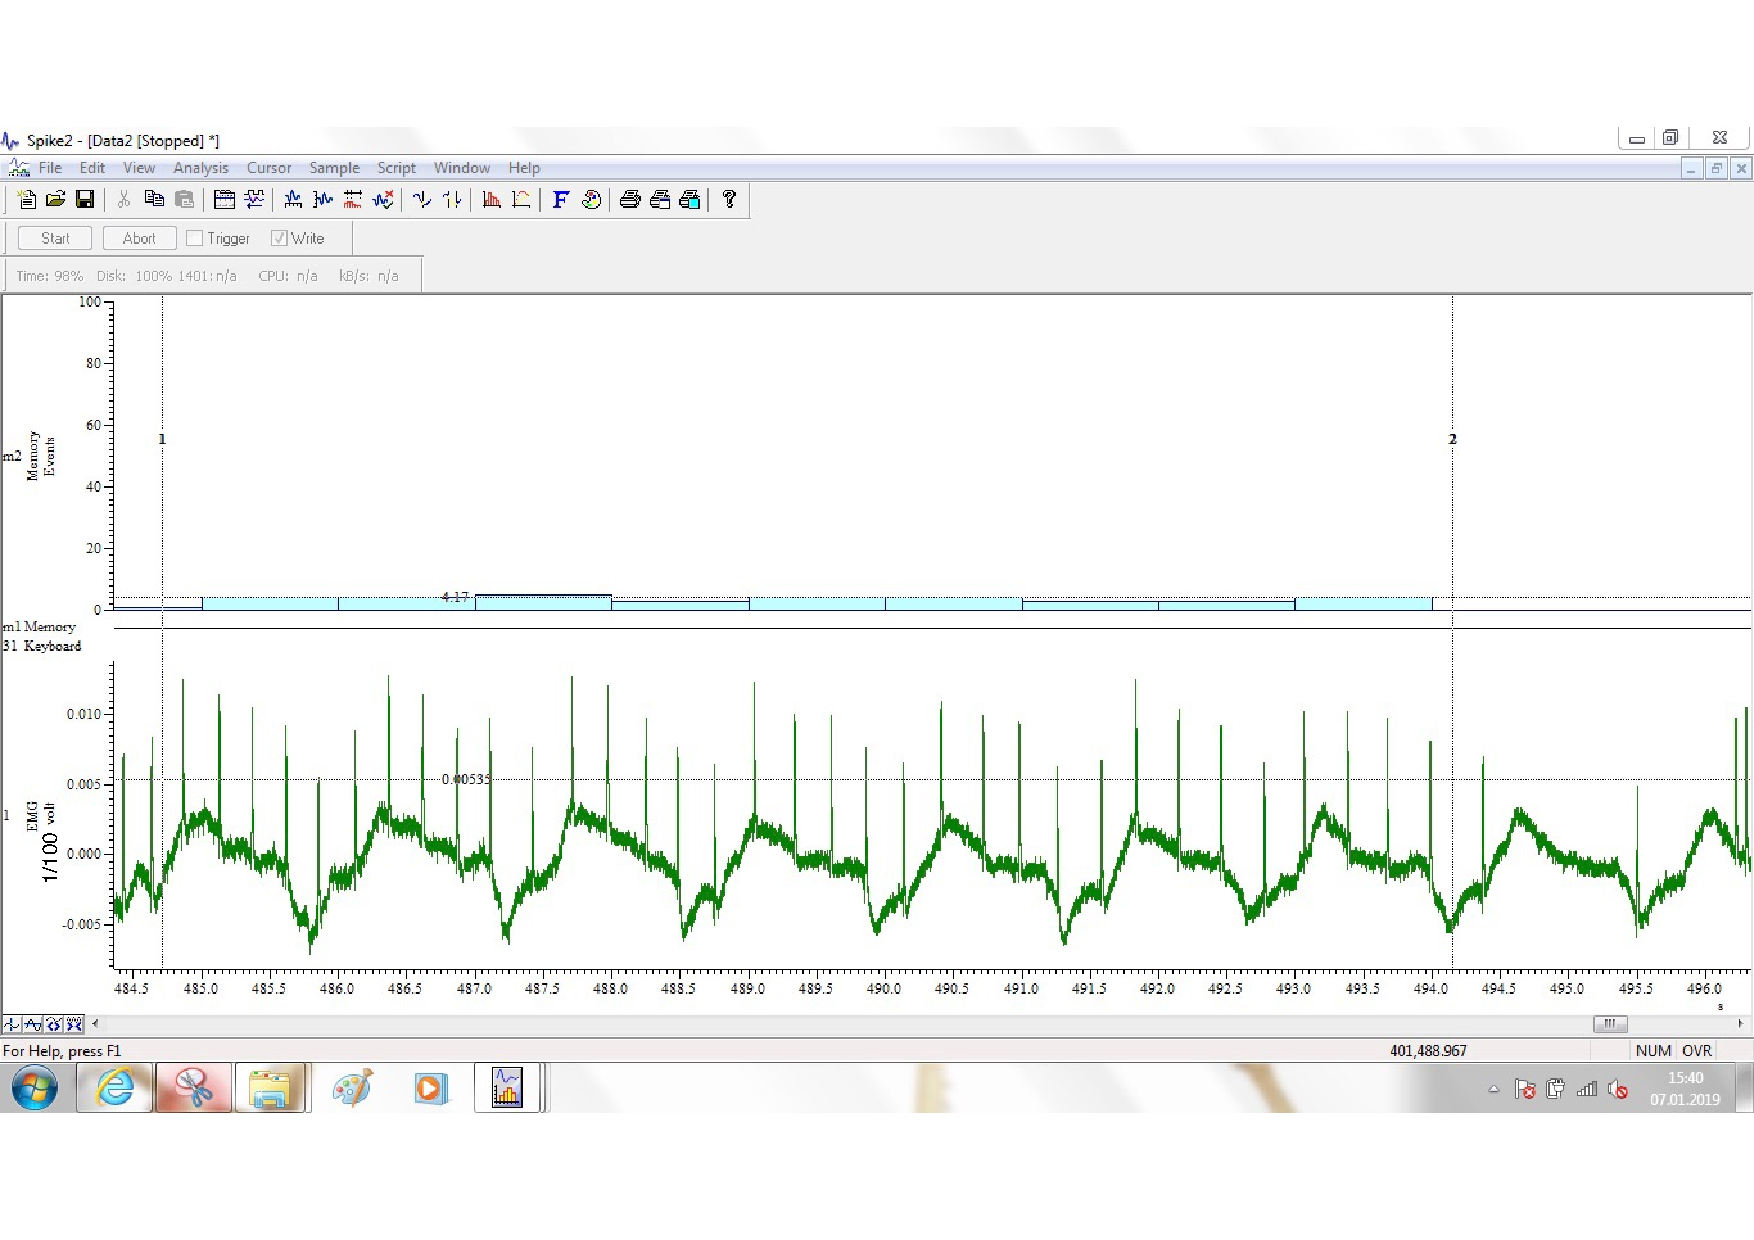
\includegraphics[width=1.3\textwidth]{kick4-1}}
\caption{EMG der Tibiastreckung}
\label{kick}
\end{figure}
Frequenz: 4.58 (s. Abb. 1)

\begin{figure}[H]
\makebox[\textwidth][c]{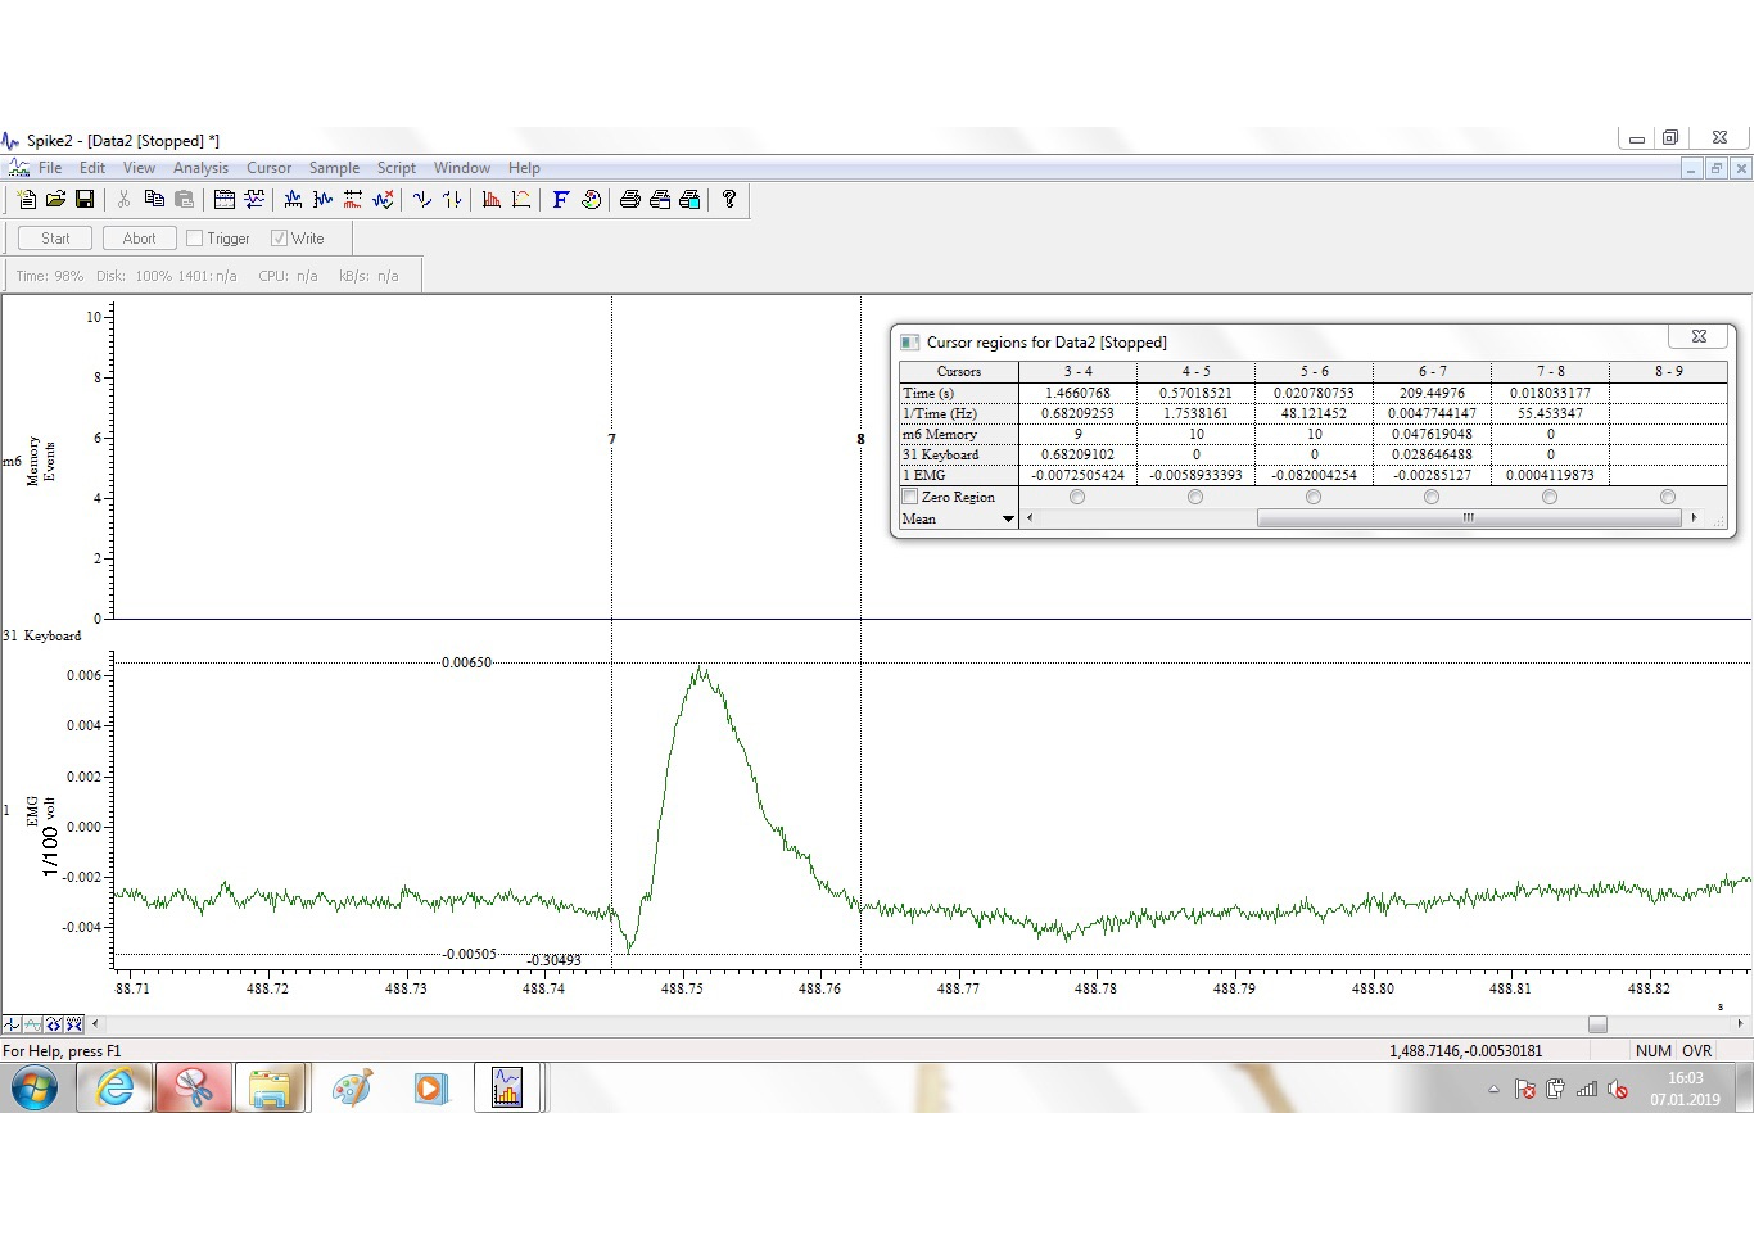
\includegraphics[width=1.3\textwidth]{kickap2-1}}
\caption{Ausgewähltes AP der Tibiastreckung}
\label{kick-ap}
\end{figure}

Dauer: 0.018/2= 0.009\\
Amplitude: 0.0128 (s. Abb. 2)

\subsection{"{}Thrusting"{}-Bewegung}
(Elektroden leider vertauscht weil rausgerutscht)
\begin{figure}[H]
\makebox[\textwidth][c]{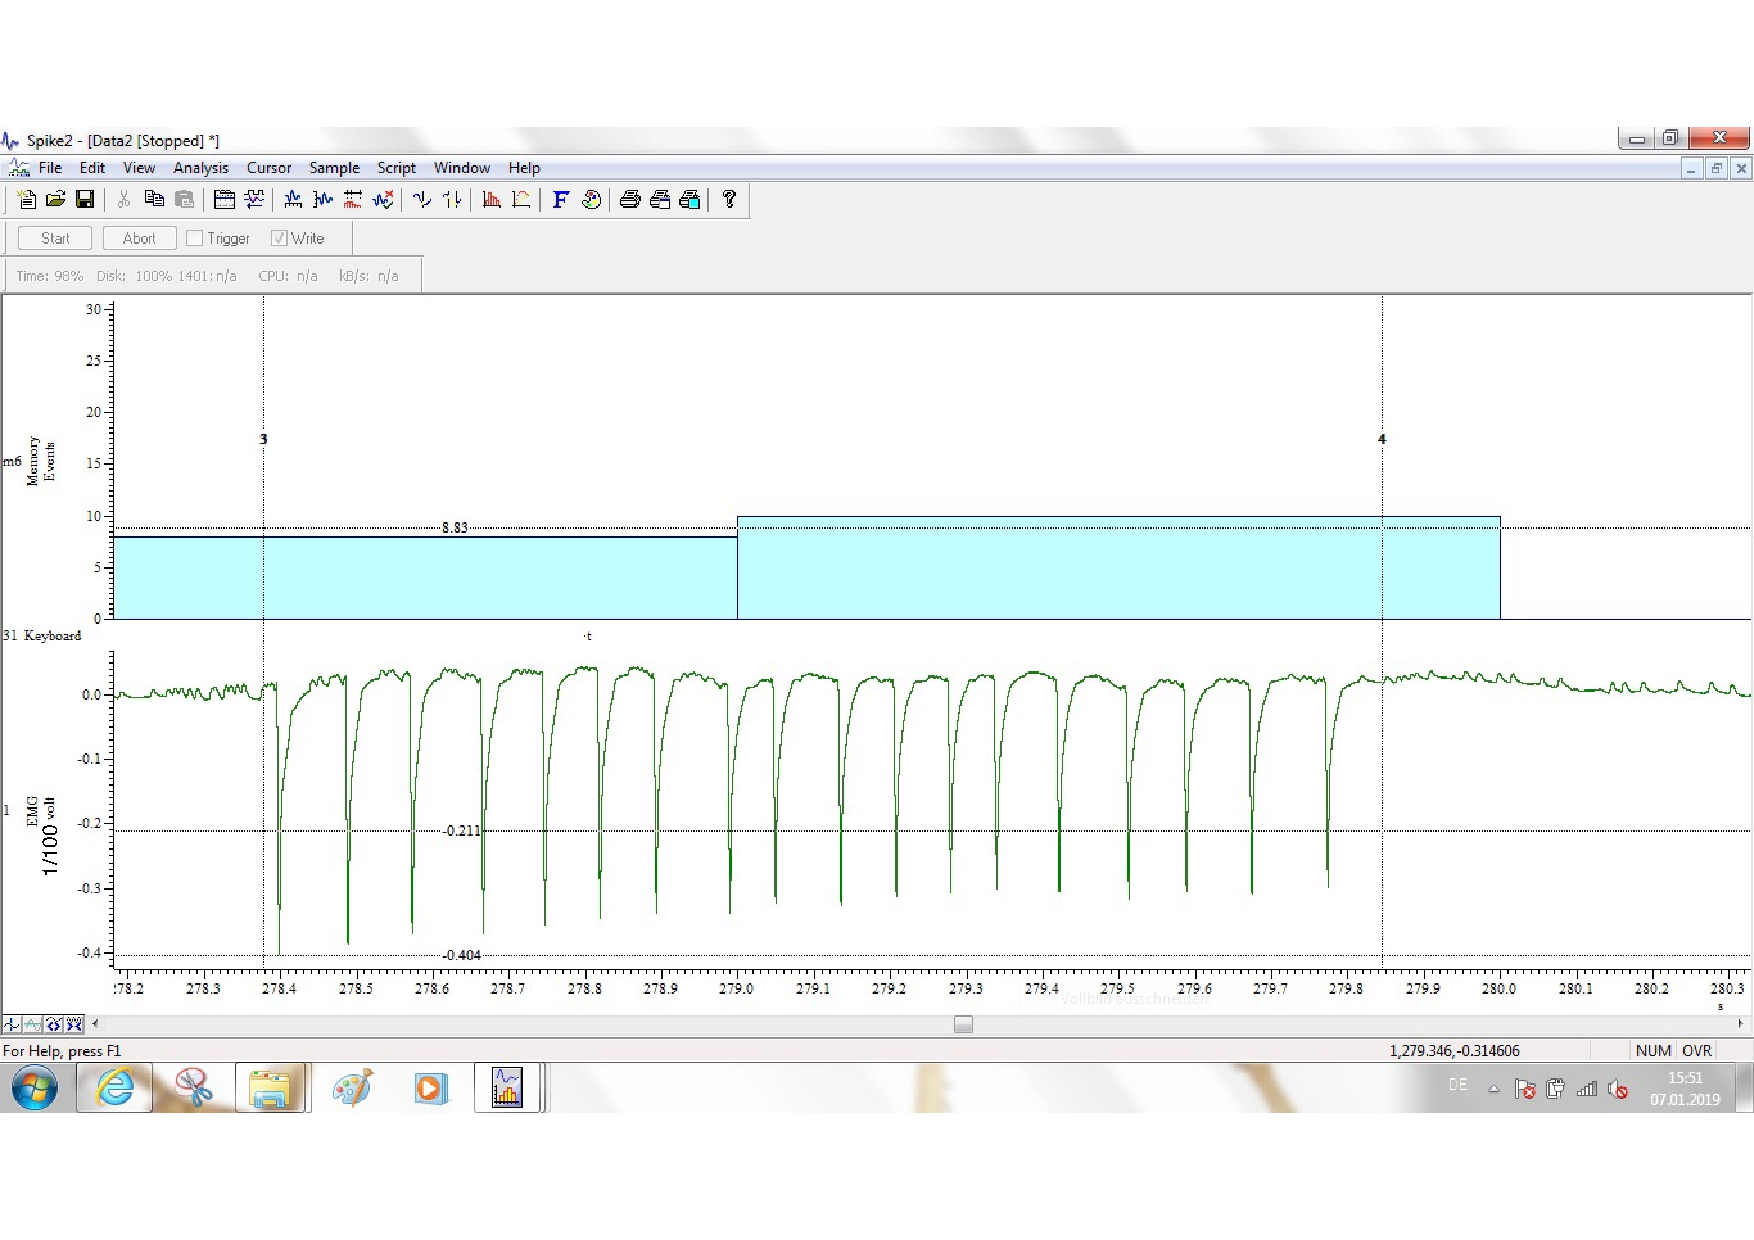
\includegraphics[width=1.3\textwidth]{thrust3-1}}
\caption{EMG der "{}Thrusting"{}-Bewegung}
\label{thrust}
\end{figure}
Frequenz: 8.83 (s. Abb. 3)

\begin{figure}[H]
\makebox[\textwidth][c]{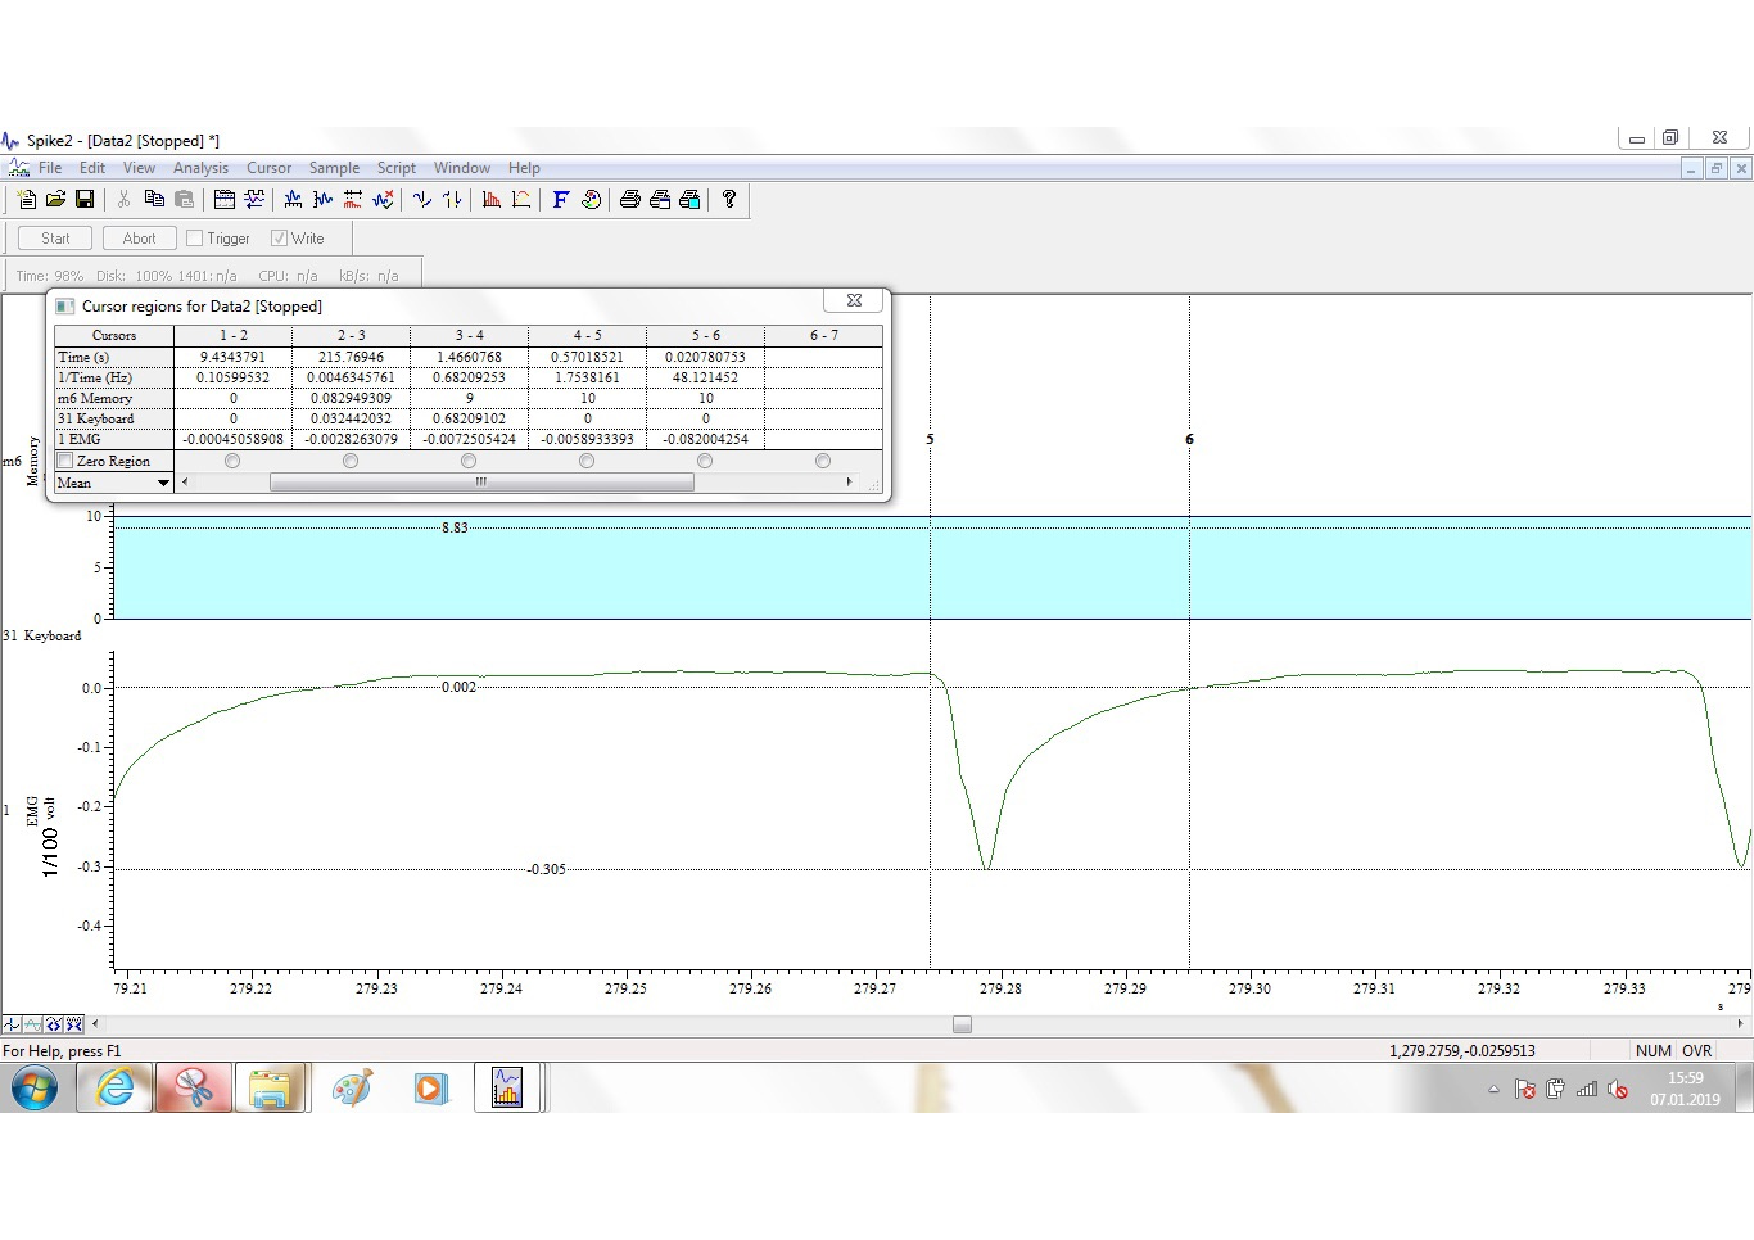
\includegraphics[width=1.3\textwidth]{thrust-AP3-1.pdf}}
\caption{Ausgewähltes AP der "{}Thrusting"{}-Bewegung}
\label{thrust-ap}
\end{figure}



Dauer: 0.0208\\
Amplitude: 0.305 (s. Abb. 4)

\section{Diskussion}
Zunächst ist für die Interpretation der gemessenen Spannungen zu betrachten, dass es sich hier um eine differentielle Ableitung im extrazellulären Bereich handelt. Das heißt es wird nicht nur die Spannung an einer Stelle betrachtet, sondern die Differenz der Spannungen zwischen den beiden Einstichen der Messelektroden im Oberschenkel der Heuschrecke. Diese Messmethode hat außerdem den Vorteil, dass Störsignale von elektromagnetischen Wechselfeldern der Umgebung eliminiert werden können, da sie sich in der Regel sehr schnell ausbreiten und somit nahezu gleichzeitig an beiden Messpunkten ankommen. Bei der Berechnung der Differenz beider Signale subtrahieren sich die Werte der Störsignale also wie folgt:
\begin{center}
$U_{ges}= (U_1+S_1) - (U_2 + S_2)$ \\

Unter der Annahme, dass $S_1 \approx S_2$, gilt: \\

$U_{ges} \approx U_1 - U_2$
\end{center}

In Abbildung 5 ist skizzenhaft die Ausbreitung eines Aktionspotenzials in Form der Ringe a) - c) gezeigt und die Messelektroden an den Stellen $1$ und $2$. Beispielhaft wird im Folgenden berechnet, welche Spannungsunterschiede man zwischen $1$ und $2$ messen würde, wenn sich das Aktionspotenzial jeweils an den Punkten a) - c) befindet: 
\begin{align*}
a)\,\, U_{ges} &= -60\mu V - 0\mu V =  -60\mu V\\
b)\,\, U_{ges} &= 0\mu V - 0\mu V =  0\mu V\\
c)\,\, U_{ges} &= 0\mu V - -60\mu V =  60\mu V\\
\end{align*}
Das Elektromyogramm würde entsprechend die Form des Graphen in Abbildung 6 annehmen. Ein Aktionspotenzial ist also "{}doppelt"{} zu sehen. 
\begin{figure}[H]
\makebox[\textwidth][c]{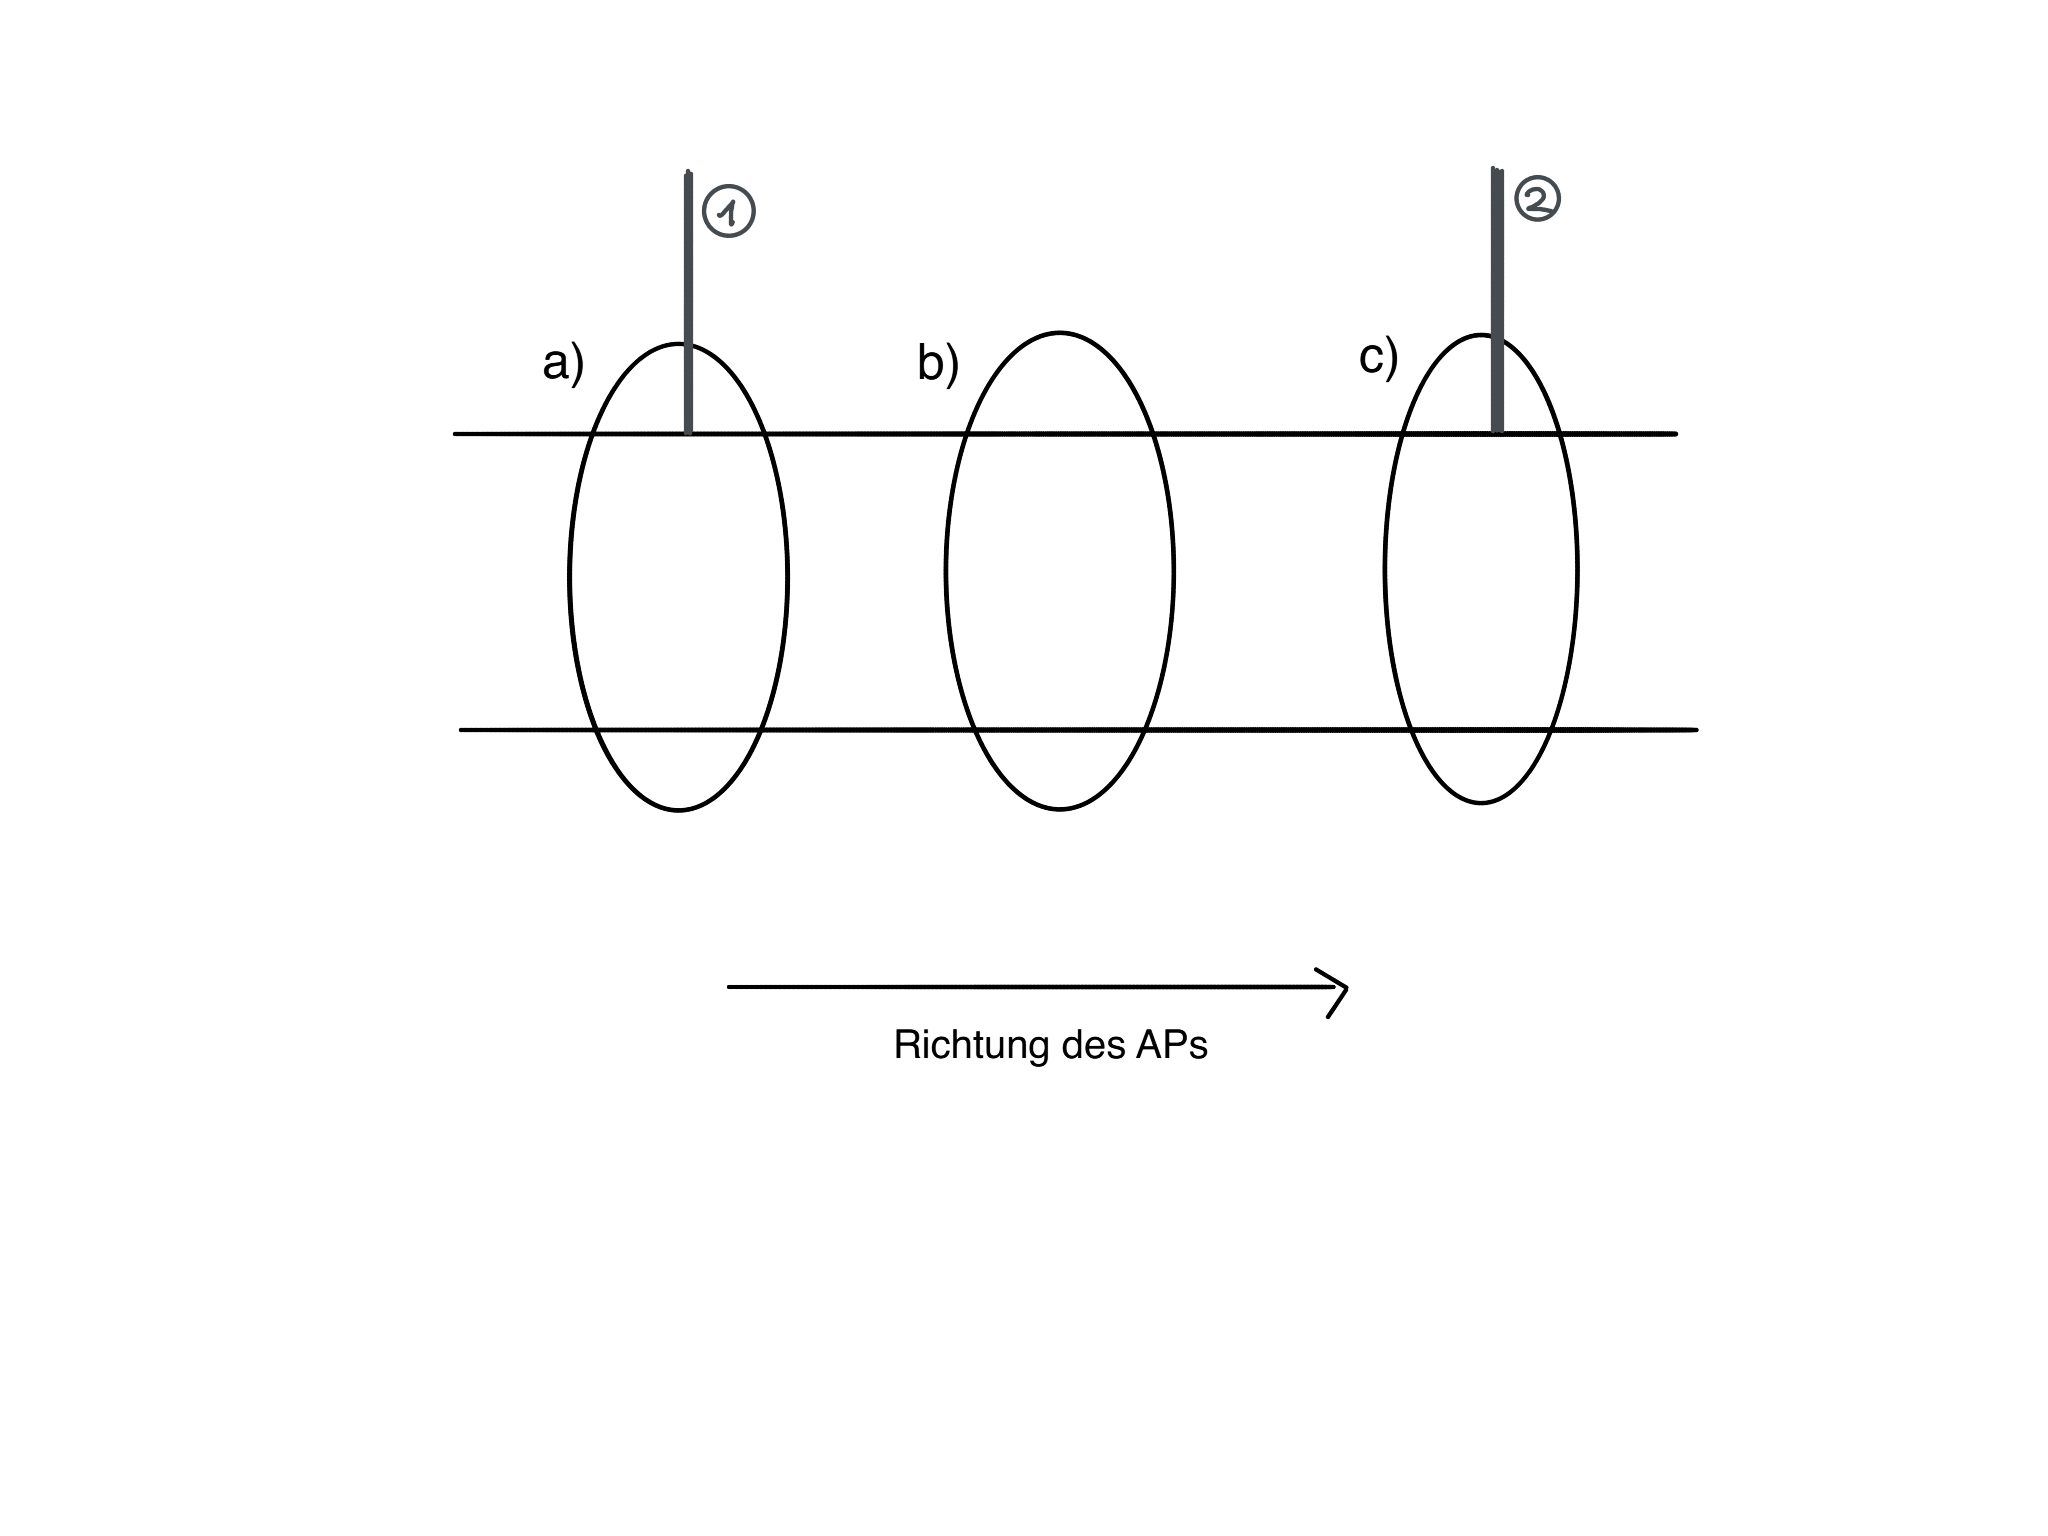
\includegraphics[width=0.9\textwidth]{diff.png}}
\caption{Skizze Elektroden und Ausbreitung des Aktionspotenzials}
\label{diff}
\end{figure}

\begin{figure}[H]
\makebox[\textwidth][c]{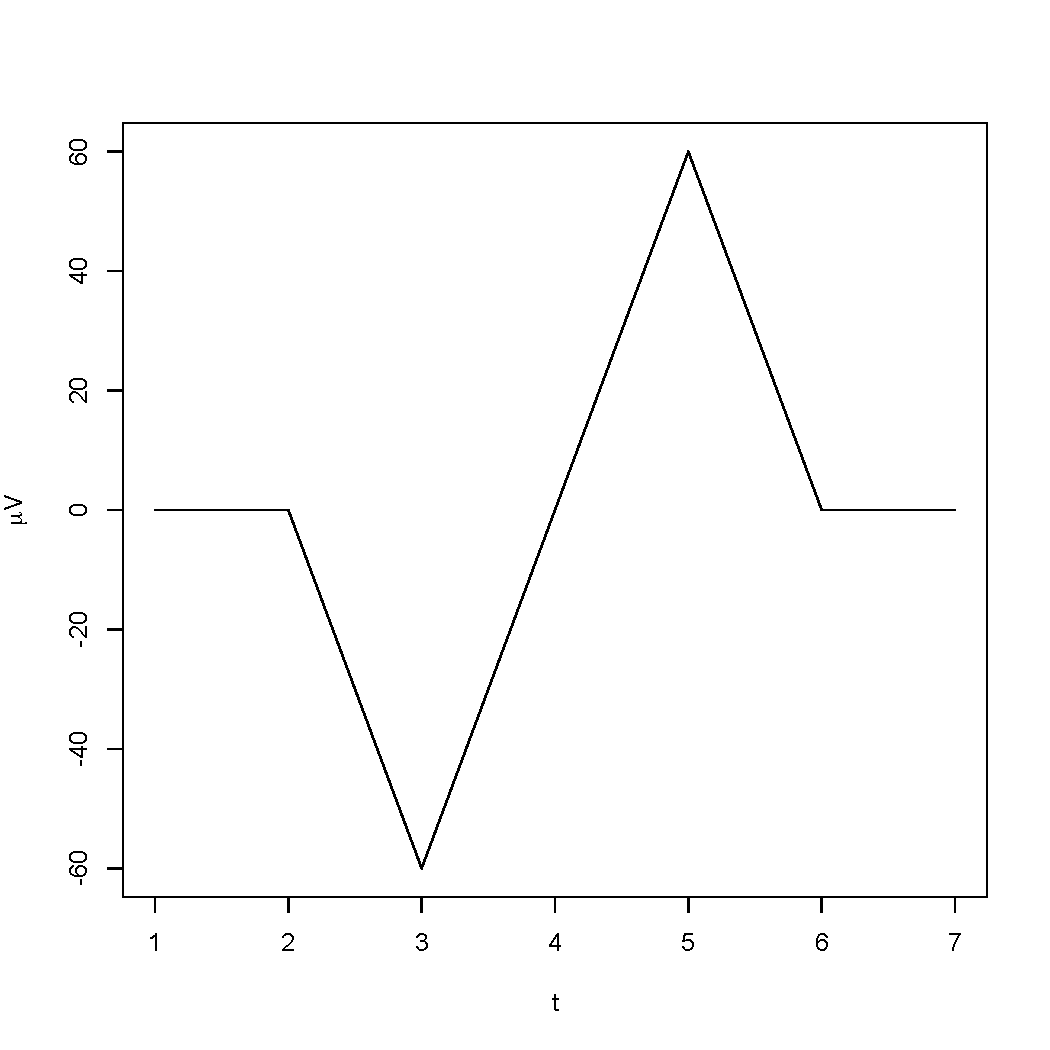
\includegraphics[width=0.8\textwidth]{plotvolt}}
\caption{Elektromyogramm Aktionspotenzial}
\label{plot_elektromyogramm}
\end{figure}

Vor der Interpretation der Ergebnisse ist zu bemerken, dass die Messdaten einige Ungenauigkeiten enthalten. \\
Idealerweise würde das aufgenomme Elektromyogramm Aktionspotenziale in Form des Beispiels in Abbildung 6 zeigen. Jedoch zeigen die Daten hauptsächlich einen Ausschlag in eine Richtung, dies könnte darauf zurückzuführen sein, dass eine Messelektrode nicht ideal im Oberschenkel plaziert wurde. Vor allem die Aufzeichnungen zum Versuch der "{}Thrusting"{}-Bewegung bilden die Spannungsdifferenz größtenteils nur in eine Richtung ab, daher wurde hier die Dauer des einzelnen Aktionspotenzials nur daraus bemessen. Im anderen Fall der "{}Kick"{}-Bewegung haben wir die Dauer beider Ausschläge halbiert, um die Dauer zu approximieren. \\
Zusätzlich ist zu berücksichtigen, dass die Elektroden im Verlauf des Versuchs ausgetauscht wurden, da sie durch unbeabsichtigte Bewegung herausgefallen sind. Dies begründet den Vorzeichenwechsel im Ausschlag der Aktionspotenziale. \\

Die Messergebnisse zu den Versuchen zeigen einen deutlichen Unterschied zwischen den Frequenzen der "{}Kick"{}- und "{}Thrusting"{}-Bewegung: die Frequenz der "{}Thrusting"{}-Bewegung (8.83) ist ca. doppelt so groß wie die Frequenz des 1. Versuchs mit der einfach Tibiastreckung (4.58) . Dies ist auf die Eigenschaften der elektromechanischen Kopplung über die langsamen Motoneurone zurückzuschließen. Es gilt, dass eine hohe Frequenz der Aktionspotenziale in den Motoneuronen zu einer dauerhaften Kontraktion des Muskels führt, wie sie im zweiten Versuch bei der "{}Thrusting"{}-Bewegung auftritt (ausgelöst durch den Widerstand). Damit der Muskel in der ausgestreckten, also angespannten Position bleibt, um gegen den Widerstand zu drücken, muss das Motoneuron in hoher Frequenz Aktionspotenziale senden.  \\

Außerdem ist zu beobachten, dass auch die Amplitude bzgl. der einzelnen betrachteten Aktionspotenziale bei der "{}Thrusting“{}-Bewegung (0.305) deutlich größer ist als die Amplitude der einfachen Tibiastreckung (0.0128). Nach dem Alles-oder-Nichts-Gesetz der Aktionspotenziale gilt, dass bei der Reizweiterleitung in Folge der Überschreitung eines Schwellenpotenzials die Intensität des Aktionspotenzials immer gleich ist. Demnach würde man hier keine Unterschiede in der Amplitude erwarten. Es handelt sich aber nicht um eine intrazelluläre, sonder eine extrazelluläre differentielle Ableitung.  Gemessen werden also Spannungsunterschiede, die aus Aktionspotenzialen mehrerer Motoneurone resultieren und sich somit zu einer größeren Spannungsdifferenz aufsummieren. Damit konnten wir zeigen, dass verschiedene Arten von Motoneuronen für die zwei verschiedenen, untersuchten Bewegungsarten verantwortlich sind, die aber den gleichen Muskel innervieren. \\
Dies ist eine typische Eigenschaft der wirbellosen Tiere: im Gegensatz zu Wirbeltieren werden bei ihnen Muskelfasern von mehreren Motoneuronen innerviert. 



%(Tafelbild.\\
%Wichtig: Messen Spannungsdifferenz zwischen den Elektroden nicht direkt AP's\\
%Thrusting durch Widerstand Dauerbelastung\\)
%(Amplitude bei Thrust höher, weil mehrere Motoneuronen die Muskelfaser aktivieren, obwohl Ap Amplitude immer gleich\\)
%(Frequenzunterschiede\\)
%AP's unsauber wegen Störungen und müden Heuschrecken.\\
%Eigentlich in beide Richtungen aber Messfehler.\\
%(Versuch zeigt, dass 2 verschiedene Arten motoneuronen innervieren  gleichen  Muskel\\)
%Amplitudenunterschied auch an Position der Elektroden und wegen extrazellulär

\end{document}

